%
%
%

\section{Top Quark Pair-Production Cross-Section Combination}

A precise measurement of the Top Quark Pair-Production Cross-Section is crucial for understanding the performance of the ATLAS detector, for testing predictions of the standard model, to searching for or constraining many new physical models.
In particle physics, a cross-section is a way to describe the rate of a specific interaction or class of interactions independently of beam conditions that are used to produce it.
The value of the top-quark pair-production cross-section in the Standard Model can be predicted using Monte-Carlo simulation techniques \cite{TOP_XSC_THEORY} \cite{TTBAR_HADRON_COLLIDERS} \cite{THRESHOLD_EXPANSION_XSC}.
This value can be determined using ``Next to Leading Order'' techniques (NLO) and is corrected by adding the ``Next to Next to Leading Order'' soft logarithm terms (approximate NNLO).
This value is determined to be $\sigma_{\ttbar} = 165^{11}_{16}$ with an uncertainty below 10\%.
The most accurate experimental determinations of the top quark's cross section previous to the LHC's results were measured by the CDS and the D0 collaborations at the Tevatron \cite{TEVATRON_XSC_LJETS} \cite{TEVATRON_XSC_DILEP}.
These experiments determined the cross-section at a center-of-mass energy of $\sqrt{s} = 7 TeV$ to a precision of 8\% using individual channels and 6.4\% by combining measurements across multiple channels.

The top-quark pair-production cross section has been measured at ATLAS using many channels and analysis technqiues.
The most precise measurements use combination of several individual measurements, which reduces both statistical and systematic uncertainties.
This section presents an ATLAS measurement of the $\ttbar$ cross-section that statistically combined three separate analysies strategies.
The likelihoods for measurements using single-lepton, dilepton, and all-hadronic channels were modeled as functions of the top cross-section, as well as a variety of nuisance parameters.
% This combination was performed by modeling the likelihoods of several individual measuremnets as functions of the top cross-section as well as a variety of nuisance parameters.
These likelihoods were then merged and a simultaneous fit to the measured data across all channels was performed.

The combined measurement of the $\ttbar$ cross-section used a measurement in the lepton+jets channel which was performed using 0.7$\ifb$ of data recorded in 2011 \cite{LEPTON_JETS_NOTE_2011}, a measurement in the dilepton channel which was performed using 0.7 $\ifb$ of data collected in 2011 \cite{DILEPTON_PAPER}, and a measurement in the all-hadronic channel, which was performed using 1.02 $\ifb$ of data collected in 2011 \cite{ALL_HADRONIC_NOTE}.


\subsection{Top Quark Pair-Production}

The primary means of producing top quarks at the LHC is via gluon fusion and subsequent decay into a pair of top quarks.

\begin{figure}
  \begin{center}

    \subfigure[Production]{
      % TopQuarkPairProductionDiagram: http://kjende.web.cern.ch/kjende/netzwerk/images/Feynman/WplusWminusBBar.png
      \includegraphics[width=.4\linewidth]{figures/xsection/TopQuarkPairProductionDiagram.png}
    }
    \subfigure[Decay]{
      % TopQuarkBranchingRatios: http://ej.iop.org/images/0034-4885/75/5/056201/Full/rpp347183f06_online.jpg
      \includegraphics[width=.4\linewidth]{figures/xsection/TopQuarkBranchingRatios.jpg}
    }
  \end{center}
  \caption{ A typical feynman diagram of top quark pair production at the LHC.  Top quarks decay into W-bosons and b-quarks nearly 100\% of the time.  The subsequent decays of the W-Bosons determine the event topology of the \ttbar event.  Diagram showing the branching ratios of Top Quark pairs into leptons and quarks.}
  \label{img:TopQuarkPairProduction}
\end{figure}

W bosons decay either leptonically, in which they produce a lepton and a neutrino, or hadronically, in which they produce a pair of quarks.
W's decay leptonically 32.6\% of the time, which consists of decaying via $W- \rightarrow e \bar{\nu_{e}}$ 10.75\% of the time, via $W- \rightarrow \mu \bar{\nu_{\mu}}$ 10.57\% of the time, and via $W- \rightarrow \tau \bar{\nu_{\tau}}$ 11.25\% of the time, and decay into quarks the other 67.60\% of the time. \cite{PARTICLE_DATA_GROUP}
% W-Boson: http://pdg.lbl.gov/2012/listings/rpp2012-list-w-boson.pdf
However, tau leptons are themselves unstable particles that subsequently decay either leptonically (muon 17.41 or electron 17.83), or hadronically 64.76\% of the time, with about 50\% of the tau's today decays into 1 hadron and 15\% into 3 hadrons.
% Tau pdg: http://pdg.web.cern.ch/pdg/2012/listings/rpp2012-list-tau.pdf
In the discussion that follows, leptonic decays of a top quark include $t \rightarrow W \rightarrow \tau \rightarrow e$ or $t \rightarrow W \rightarrow \tau \rightarrow \mu$, and we will ignore the intermediate state $\tau$ in terms of our classification.
Hence, a pair of top quarks, which we assume always decay into a pair of W bosons, will decay into two leptons 6.5\% of the time (known as the ``dilepton'' channel), into a single lepton and a pair of quarks 34.4\% of the time (known as the ``single lepton'' channel), and entirely into quarks 45.7\% of the time (known as the ``all hadronic'' channel).
% pdg:
% Citation: J. Beringer et al. (Particle Data Group), PR D86, 010001 (2012) (URL: http://pdg.lbl.gov)



%% \begin{figure}
%%   \begin{center}
%%     % TopQuarkBranchingRatios: http://ej.iop.org/images/0034-4885/75/5/056201/Full/rpp347183f06_online.jpg
%%     \includegraphics[width=100mm]{figures/xsection/TopQuarkBranchingRatios.jpg}
%%   \end{center}
%%   \caption{}
%%   \label{img:TopQuarkBranchingRatios}
%% \end{figure}

\subsection{Object Reconstruction}

Measurements of $\ttbar$ event require kinematicaly reconstructing and selecting a variety of physical objects, including electrons, muons, jets, b-jets, and $\MET$.

% Selected Electrons
Selected electrons are required to have a calorimeter cluster located in a pseudorapidity range of $0 < |\eta| < 4.47$, excluding the range $1.37 < |\eta| < 1.52$ (this excluded interval, known as the crack region, is a mostly un-insturmented part of the EM calorimeter).
To reject jets that fake electrons, the electron's energy is required to be isolated in the calorimeter.
Specifically, electrons with more than 3.5 GeV of energy in a cone of $\sqrt{(\Delta \eta)^2 + (\Delta \phi)^2}$, excluding the energy of the electron itself, are rejected.
Electrons must pass a variety of cuts related to the shape of its shower and the quality of its corresponding track that are collectively referred to as ``tight'' EM identification cuts.
Finally, Electrons must have a minimum energy of $E_{T} > 20$ GeV, where $E_{T}$ referrs to the transverse energy of the electron's electromagnetic cluster..

%% The selection of l + jets tt ̄ events makes use of reconstructed electrons, muons and jets, and the transverse momentum imbalance referred to as missing transverse energy Emiss.
%% T Electron candidates are reconstructed from the energy depositions in the electromagnetic calorimeter
%% and are required to have a well-measured track associated with the electromagnetic cluster. The latter is required to have |ηcluster| < 2.47 excluding 1.37 < |ηcluster| < 1.52 corresponding to the transition region between barrel and endcap calorimeters. To ensure that electrons are isolated from the jet activity, as expected for prompt electrons from W boson decay, the energy in a cone of ∆R ≡ 􏰮∆η2 + ∆φ2 = 0.2, centered around the electron, excluding the energy associated with the electron itself, is required to be < 3.5 GeV. This defines the tight electron candidates used for the final analysis. Loose electron candidates employed for the estimation of the QCD multijet background, as described in Section 4, have to fulfill less stringent requirements and the isolation cut is increased to < 6 GeV energy deposition in ∆R = 0.2.

% Selected Muons
Selected Muons must be ``combined'', meaning they must use tracks from both the muon spectrometer and the inner detector.
Only muons within $|\eta| < 2.5$ are considered, and muons within $\Delta R <= 0.4$ of a selected jet are rejected.
Two isolation requirements are imposed on selected muons.  
They must be isolated in the calorimeter, meaning the energy deposited in the calorimeter within $\Delta R = 0.3$ must be $<$ 4 GeV, and their tracks must be isolated, meaning the sum of the transverse momenta of tracks in a code of $\Delta R = 0.3$ surronding the muon's track must be $<$ 4 GeV.

%% Muon candidates are reconstructed by searching for track segments in the different layers of the muon spectrometer. These segments are then combined starting from the outermost layer, and matched with the inner detector tracks. The final parameters of muon candidates are obtained from the combined fit using information from both detector systems. Only muons within |η| < 2.5 are included in this measurement. Like electrons, muons are required to be isolated, i.e. (i) be separated from the closest jet by ∆R(μ, jet) > 0.4; (ii) have calorimeter isolation < 4 GeV and (iii) have track isolation < 4 GeV. Track isolation is defined as the sum of track transverse momenta in a cone ∆R ≡ 􏰮∆η2 + ∆φ2 = 0.3, excluding the pT of the muon track, while calorimeter isolation is defined as energy deposition in the calorimeter within a cone of ∆R = 0.3, excluding the energy deposition directly along the muon track. Muons passing all requirements are used in the analysis sample selection and are referred to as tight, while muons with a looser isolation are used for the QCD multijet background estimate described in Section 4. In this case, all requirements except the cuts on calorimeter and track isolation have to be fulfilled and the muons are referred to as loose.

% Selected Jets
In this analysis, Jets are constructed using the anti-kt algorithm with a distance parameter of $R=0.4$.
These jets are built out of ``topoligical clusters'', which themselves are collections of neighboring cells that each have an energy above some threshold, where the energy has been calibrated to the scale of electromagnetic showers (known as ``Electromagnetic Scale'').
Once the jets are built, their energies are then recalibrated to the scale of hadronic particles (known as the ``Hadronic scale'') \cite{JES_SCALE_2010}.
Since jets are built out of calorimeter deposits, essentially all electrons will also be reconstructed as jets.
Therefore, these objects must be removed from the collection of selected jets by-hand.
In this analysis, any jet that overlaps with a selected electron within $\Delta R < 0.2$ is removed.

%% Jets are reconstructed using the anti-kt algorithm with distance parameter R = 0.4 [9] which sets the relative distance at which jets are resolved from each other. As input, the algorithm uses topological clusters that group together neighboring calorimeter cells with energy deposits above certain thresholds. Their energy accounts correctly for the energy deposited in the calorimeter by electromagnetic showers. Additional correction factors dependent on jet η and pT are applied to the reconstructed jets to correct their energy to the hadronic scale. The jet energy scale (JES) is established using corrections derived from collision and test beam data and calibration constants obtained from MC simulation [10]. Since reconstructed electrons might also be reconstructed as jets in the calorimeter, any jet overlapping with a %% 2 %% tight electron within a cone of ∆R < 0.2 is removed from the list of jets. 

%% MET
Finally, once all objects have been selected, the $\MET$ is defined as the vector sum of the calorimeter energy deposits of selected objects or the combined energy for muons (including additional corrections for energy deposited in the calorimeter).
The energy associated with each object is calibrated to the scale of that object, and all remaining energy deposits are added to the $\MET$ vector, but at electromagnetic scale.

%% The analysis reconstructs the missing transverse energy from the vector sum of energy depositions
%% in the calorimeter in the transverse plane associated to the objects used in the analysis. The same recon-
%% struction and identification algorithms as for the analysis objects are used to identify electrons and jets.
%% The corresponding topological clusters in the calorimeters are then included in the calculation of Emiss at T
%% the energy scale of the associated object. The muon momenta are calculated using the information from both the inner detector and the muon spectrometer system and corrected for additional energy deposi- tion in the calorimeter. Remaining energy depositions not associated to any object are included at the electromagnetic energy scale.

%% END

\subsection{Lepton+Jets}
The lepton$+$jets channel is the most statistically powerful decay of the $\ttbar$ system for measuring the pair-production cross-section.
The leptonic decay of one of the top results in an event topologiy that allows for strong background discrimination, while the hadronic decay of the other top maintains a high branching ratio for this channel.
The distinguishing features of the lepton$+$jets channel is the presence of a high-pt lepton from the leptonic decay of a W boson,v$\MET$ from a neutrino, two b-jets from the decay $t \rightarrow W+b$, and two additional jets from the hadronic decay of a W boson.
This topology of event was selected for by first requiring a single lepton trigger, which either required an electron or a muon (reconstructed by the trigger) with $E_{T} > 20 GeV$ or $p_{T} > 18 GeV$, respectively.
The exact trigger required varied throught the run periods of 2011 as higher instintaneous luminosities required stricter lepton definitions to maintain a steady bandwidth of recorded events as selected by the trigger.
Selected events are required to have a primary vertex that consists of 5 or more tracks.
Each event must have exactly 1 selected electron or muon, and that lepton must match a corresponding object that fired a single-lepton trigger (events with more than 1 lepton fall into the dilepton channel, to be described in detail later).
The energy requirements for these objects were chosen to minimize any effects resulting from the trigger's online reconstruction.
A cut on $\MET$ is imposed, requiring $\MET > 35 GeV$ for the electron channel and $\MET > 25 GeV$ for the muon channel (the difference in the cut results from different background contributions to each channel from QCD events, which tend to have low values of $\MET$).
Additional cuts are made on the to reduce the contamination from QCD, which use a variable known as the ``W boson transverse mass'':
\begin{equation}
  m_{T}(W) = \sqrt(2 p_{T}^{l} p_{T}^{\nu} (1 - cos( \phi^{l} - \phi^{\nu}))),
\end{equation} 
where the $\MET$ vector is used to determine the kinematic variables of the neutrino, $p_{T}^{\nu}$ and $\phi^{\nu}$.
Using this definition, the event selection requires $m_{T}(W) > 25 GeV$ in the electron channel or $\MET + m_{T}(W) > 60 GeV$ in the muon channel.



\subsubsection{Backgrounds}
A selection of events based on the above criteria will be contaminated with several sources of backgrounds, including

\begin{itemize}
\item QCD Multijet events where a lepton is faked via a background mechanism
\item $W+Jets$ events where the W decays leptonically (leading to $\MET$) which includes real or fake b-jets
\item $Z+Jets$ events where one of the two leptons isn't identified and which includes real or fake b-jets
\item Diboson Events (WW, WZ, or ZZ events), that include some combination of leptonic decays of vector bosons, additional jets, and real or faked b-jets
\item Single Top events
\end{itemize}

% Add figures

\begin{figure}
  \begin{center}
    \subfigure[$W+Jets$]{
      % 
      \includegraphics[width=.4\linewidth]{figures/xsection/ZJetsDiagram.png}
    }
    \subfigure[$QCD$]{
      %ZJetsDiagram.png : http://inspirehep.net/record/871058/files/qg_qZ.png
      \includegraphics[width=.4\linewidth]{figures/xsection/ZJetsDiagram.png}
    } \\
    \subfigure[$Z+Jets$]{
      %ZJetsDiagram.png : http://inspirehep.net/record/871058/files/qg_qZ.png
      \includegraphics[width=.4\linewidth]{figures/xsection/ZJetsDiagram.png}
    }
    \subfigure[$Single Top$]{
      % 
      \includegraphics[width=.4\linewidth]{figures/xsection/ZJetsDiagram.png}
    } \\
  \end{center}
  \caption{Feynman diagrams for the most important backgrounds to $\ttbar$ events.  Shown are $Z+Jets$ events (top, left), $W+jets$ events (top, right), QCD events (bottom, left) and Single Top events (bottom, right).}
  \label{img:BackgroundsFeynmanDiagrams}
\end{figure}

To measure the cross-section, the background contributions due to each of the above processes in the lepton+jets channel were determined using a variety of techniques.
The dominant $W+Jets$ background as well as the $Z+Jets$, diboson, and single-top background are estimated using Monte-Carlo simulation.
While the kinematic distributions of each $W+Jets$ event were estimated from Monte-Carlo, the expected number of events was extracted using a data-driven technique.
The technique used to estimate the normalization of the $W+Jets$ background is based on one used in a top-quark charge-asymmetry analysis \cite{CHARGE_ASYMMETRY}.
It is based on the fact that $W^{+}$ bosons are produced at a higher rate than $W^{-}$ bosons due to the fact that the LHC collides protons (and not anti-protons).
The ratio of the production of $W^{+}$ to $W^{-}$, $r_{MC}$, can be estimated using Monte-Carlo.  Assuming that $W+Jets$ events are the dominant category of events that are asymmetric between positive and negative leptons, one can estimate the total number of $W+Jets$ events by taking the difference between the measured jumber of events with a positive lepton and the number with a negative lepton:

\begin{equation}
  N_{W^{+}} + N_{W^{-}} = \frac{r_{MC} + 1}{r_{MC} - 1}(D^{+} - D^{-}),
\end{equation}

where $D^{+}$ and $D^{-}$ are the number of selected single-lepton events with a positive or negative lepton, respectively.
The value of $r_{MC}$ is measured to be 1.56 $\pm$ 0.07 for the electron channel and 1.66 $\pm$ 0.06 for the muon channel.
Estimates of overall yields or kinematic variables for the $W+Jets$ background are then weighted to a total normalization given by this data-driven value.
The normalizations for the $Z+Jets$, diboson, and single-top backgrounds are taken directly from cross-sections evaluated using monte-carlo and scaled to the integrated luminosity recorded by the ATLAS detector.

Each of the backgrounds which are estimated using Monte-Carlo lead to real leptons in the final state.
In contrast, the QCD background enters the single-lepton channel when a final state jet is falsely identified as a lepton.
The process of a jet faking a lepton depends on the details of the jet's hadronic shower, in particular it's shape and depth in both the electromagnetic and hadronic calorimeters.
The hadronic shower evolution is of course modeled in detail by simulations used by ATLAS.
However, small differences in the nature of that simulation can lead to significant changes in the rate of jets faking leptons.
And because the number of QCD events created at ATLAS is extremely large, changes in the rate will have dramatic differences in the number of background events in the lepton+jets signal region.
For this reason, it is preferable to estimate the background contribution due to QCD without relying on the details of the Monte-Carlo description of hadronic shower evolution.

The lepton+jets analysis uses a technique to extract the rate and distribution of QCD events from data directly.
Known as the ``Matrix Method,'' this technique exploits the fact that the efficiencies of real and fake leptons differ as a function of cuts on the reconstructed lepton's isolation and shower shape.
The technique involves creating two subsets of lepton identifications, denoted as ``loose'' and ``tight'' (with ``tight'' corresponding to the nominal selection requirements).
The Matrix Method relies on knowing the effecienciy for both real and fake leptons which pass loose selection to also pass the tight selection.

\begin{equation}
  \epsilon_{real} = \frac{N^{tight}_{real}}{N^{loose}_{real}} and \epsilon_{fake} = \frac{N^{tight}_{fake}}{N^{loose}_{fake}},
\end{equation}

where $N^{tight}$ and $N^{loose}$ represent the number of events with tight or loose (and not tight) lepton, respectively, in the region of phase space where the efficiency is being measured.
Given these values, one can write a set of equations relating the number of events with a measured loose or tight lepton to the number  

\begin{eqnarray}
  \bar{N^{tight}} = \epsilon_{real} N_{real} + \epsilon_{fake} N_{fake} \\
  \bar{N^{loose}} = (1-\epsilon_{real}) N_{real} + (1-\epsilon_{fake}) N_{fake}.
  \label{eq:MatrixMethod}
\end{eqnarray}

The above equations can be inverted to obtain $N_{fake}$ and $N_{real}$, quantities we're interested in estimating, as a function of  $N^{tight}$ and $N^{loose}$, quantities that can be measured.
By solving and isolating the variables $N^{tight}_{real}$ and $N^{tight}_{fake}$ (which represent the real and fake lepton contributions to the tight, or signal, region), and expressing the solution as a matrix, we obtain the following:

\begin{eqnarray}
  N^{tight}_{real} = \frac{N^{tight} - \epsilon_{fake}N^{loose}}{\epsilon_{fake} - \epsilon_{real}} \\
  N^{tight}_{fake} = \frac{\epsilon_{real}N^{loose} - N^{tight}}{\epsilon_{fake} - \epsilon_{real}}
\end{eqnarray}

\begin{equation}
\begin{pmatrix} N^{tight}_{real} \\ N^{tight}_{fake} \\ \end{pmatrix} 
  = 
  \begin{pmatrix} 
    \frac{\epsilon_{real}}{\epsilon_{real} - \epsilon_{fake}} & \frac{-\epsilon_{real}\epsilon_{fake}}{\epsilon_{real} - \epsilon_{fake}} \\ 
    \frac{-\epsilon_{fake}}{\epsilon_{real} - \epsilon_{fake}} & \frac{\epsilon_{real}\epsilon_{fake}}{\epsilon_{real} - \epsilon_{fake}} \\ 
  \end{pmatrix}  
  \begin{pmatrix} N^{tight} \\ N^{loose} \\ \end{pmatrix}
  \label{eq:MatrixMethodInverted}
\end{equation}

One should note that the solution is linear in the number of tight or loose events.
In particular, this means that we can associate any given event (be it loose or tight) with a weight for real or fake, and these weights are simply the (1,1) and (2,1) elements of the matrix in equation \ref{eq:MatrixMethodInverted}.
Therefore, in the case that the $\epsilon$ values are functions of arbitrary variables associated with an event, one can still estimate the number of fakes in the tight (signal) region as:

\begin{equation}
  N^{tight}_{fake} = \sum_{e \in tight} (\frac{-\epsilon_{fake}}{\epsilon_{real} - \epsilon_{fake}}) + \sum_{e \in loose} (\frac{\epsilon_{real}\epsilon_{fake}}{\epsilon_{real} - \epsilon_{fake}})
  \label{eq:MatrixMethodSum}
\end{equation}

Equation \ref{eq:MatrixMethodSum} is used to estimate the amount of QCD multijet events that enter the signal region (assuming that all fakes in the loose or tight regions come from QCD Multijet events).
In that estimation, loose electrons are defined identically as tight electrons, except their isolation cut is relaxed, requiring that $E_{T} < 6 GeV$ in a cone defined by $\Delta R = 0.2$.
Similarly, loose muons are identical to tight muons, but the cuts on $E_{T}$ and $p_{T}$ isolation are removed entirely.
The efficiencies for loose leptons, as defined above, to also pass tight requirements for both real and fake muons are measured directly in data.
To measure the efficiencies of real leptons, a collection of events dominated by $Z->ee$ or $Z->\mu\mu$ is created by selecting dilepton events where the invariant mass of the leptons is close to the mass of the Z-boson.
In such a sample, the efficiency can be measured directly.
For fake leptons, a sample of QCD multijet events is collected by selecting events with a single (loose) lepton, a jet, and by requiring $5 GeV < \MET <  60 GeV$ for electron events or $m_{T}(W) < 20 GeV$ and $m_{T}(W) + \MET < 60 GeV$ for muon events.
For muons, the efficiencies were paramaterized as a function of the muon's $p_{T}$ and $\eta$.
Contributions from $Z+Jets$ and $W+Jets$ in the QCD control regions were subtracted using Monte-Carlo estimates.

% e + Jets
\begin{table}
  \begin{tabular}{lccccc}
    \hline
    $e + Jets$ & 1 Jet & 2 Jet & 3 Jet & 4 Jet & $>=$ 5 Jets \\ 
    \hline
    $\ttbar$ & $225 \pm 15$ & $1005 \pm 32$ & $1934 \pm 44$ & $1835 \pm 43$ & $1463 \pm 38$ \\
    $W+Jets$ & $161600 \pm 400$ & $43170 \pm 210$ & $10840 \pm 100$ & $2486 \pm 50$ & $1032 \pm 32$ \\
    $QCD Multijets$ & $11000 \pm 5000$ & $4800 \pm 2400$ & $1600 \pm 800$ & $510 \pm 250$ & $117 \pm 89$ \\
    Single Top & $571 \pm 24$ & $711 \pm 27$ & $391 \pm 20$ & $156 \pm 13$ & $65 \pm 8$ \\
    $ZJets$ & $3732 \pm 61$ & $2444 \pm 49$ & $996 \pm 32$ & $333 \pm 18$ & $146 \pm 12$ \\
    Diboson & $599 \pm 25$ & $538 \pm 23$ & $178 \pm 13$ & $45 \pm 7$ & $10 \pm 3$ \\
    \hline
    Total Predicted & $177000 \pm 5000$ & $52600 \pm 2400$ & $15900 \pm 800$ & $5360 \pm 260$ & $2892 \pm 100$ \\
    Total Observed & 179469 & 51820 & 15614 & 5398 & 2812 \\
    \hline
  \end{tabular}
  \caption{Predicted and observed event yields in bins of jet number for the $\ttbar$ signal and backgrounds in the $e+jets$ channel.  Yields are obtained using Monte Carlo or Data-Driven techniques, depending on the sample.}
\end{table}

% mu + Jets
\begin{table}
  \begin{tabular}{lccccc}
    \hline
    $e + Jets$ & 1 Jet & 2 Jet & 3 Jet & 4 Jet & $>=$ 5 Jets \\ 
    \hline
    $\ttbar$ & $319 \pm 18$ & $1342 \pm 37$ & $2734 \pm 52$ & $2714 \pm 52$ & $2030 \pm 45$ \\
    $W+Jets$ & $383200 \pm 600$ & $93440 \pm 310$ & $20140 \pm 140$ & $4644 \pm 68$ & $1082 \pm 33$ \\
    $QCD Multijets$ & $25000 \pm 12000$ & $11000 \pm 6000$ & $3200 \pm 1600$ & $900 \pm 400$ & $290 \pm 150$ \\
    Single Top & $996 \pm 32$ & $1148 \pm 34$ & $594 \pm 24$ & $210 \pm 15$ & $84 \pm 9$ \\
    $ZJets$ & $17270 \pm 130$ & $5492 \pm 74$ & $1510 \pm 39$ & $436 \pm 21$ & $149 \pm 12$ \\
    Diboson & $1093 \pm 33$ & $1009 \pm 32$ & $308 \pm 18$ & $69 \pm 8$ & $18 \pm 4$ \\
    \hline
    Total Predicted & $428000 \pm 12000$ & $113000 \pm 6000$ & $28400 \pm 1600$ & $8900 \pm 400$ & $3660 \pm 160$ \\
    Total Observed & 433931 & 111741 & 28643 & 8680 & 3814 \\
    \hline
  \end{tabular}
  \caption{Predicted and observed event yields in bins of jet number for the $\ttbar$ signal and backgrounds in the $\mu+jets$ channel.  Yields are obtained using Monte Carlo or Data-Driven techniques, depending on the sample.}
\end{table}


\begin{figure}
  \begin{center}
    \subfigure[$e+jets$] {
      % EJetsYieldPlot.eps: https://atlas.web.cern.ch/Atlas/GROUPS/PHYSICS/CONFNOTES/ATLAS-CONF-2011-121/fig_01a.eps
      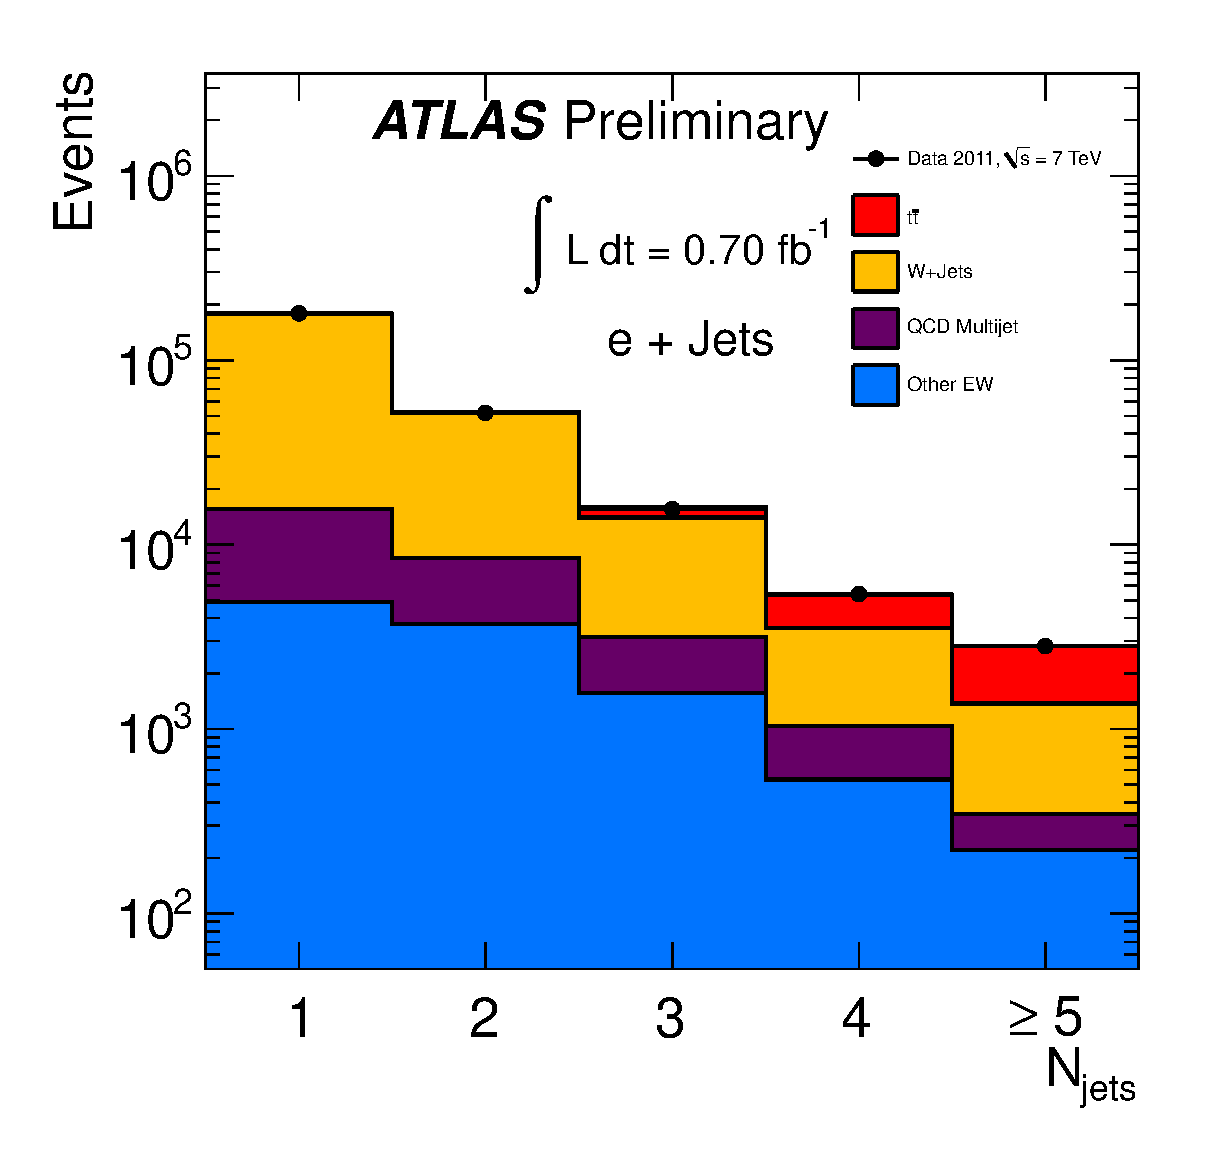
\includegraphics[width=.45\linewidth]{figures/xsection/EJetsYieldPlot}
    }
    \subfigure[$\mu+Jets$] {
      % MuJetsYieldPlots.eps: https://atlas.web.cern.ch/Atlas/GROUPS/PHYSICS/CONFNOTES/ATLAS-CONF-2011-121/fig_01b.eps
      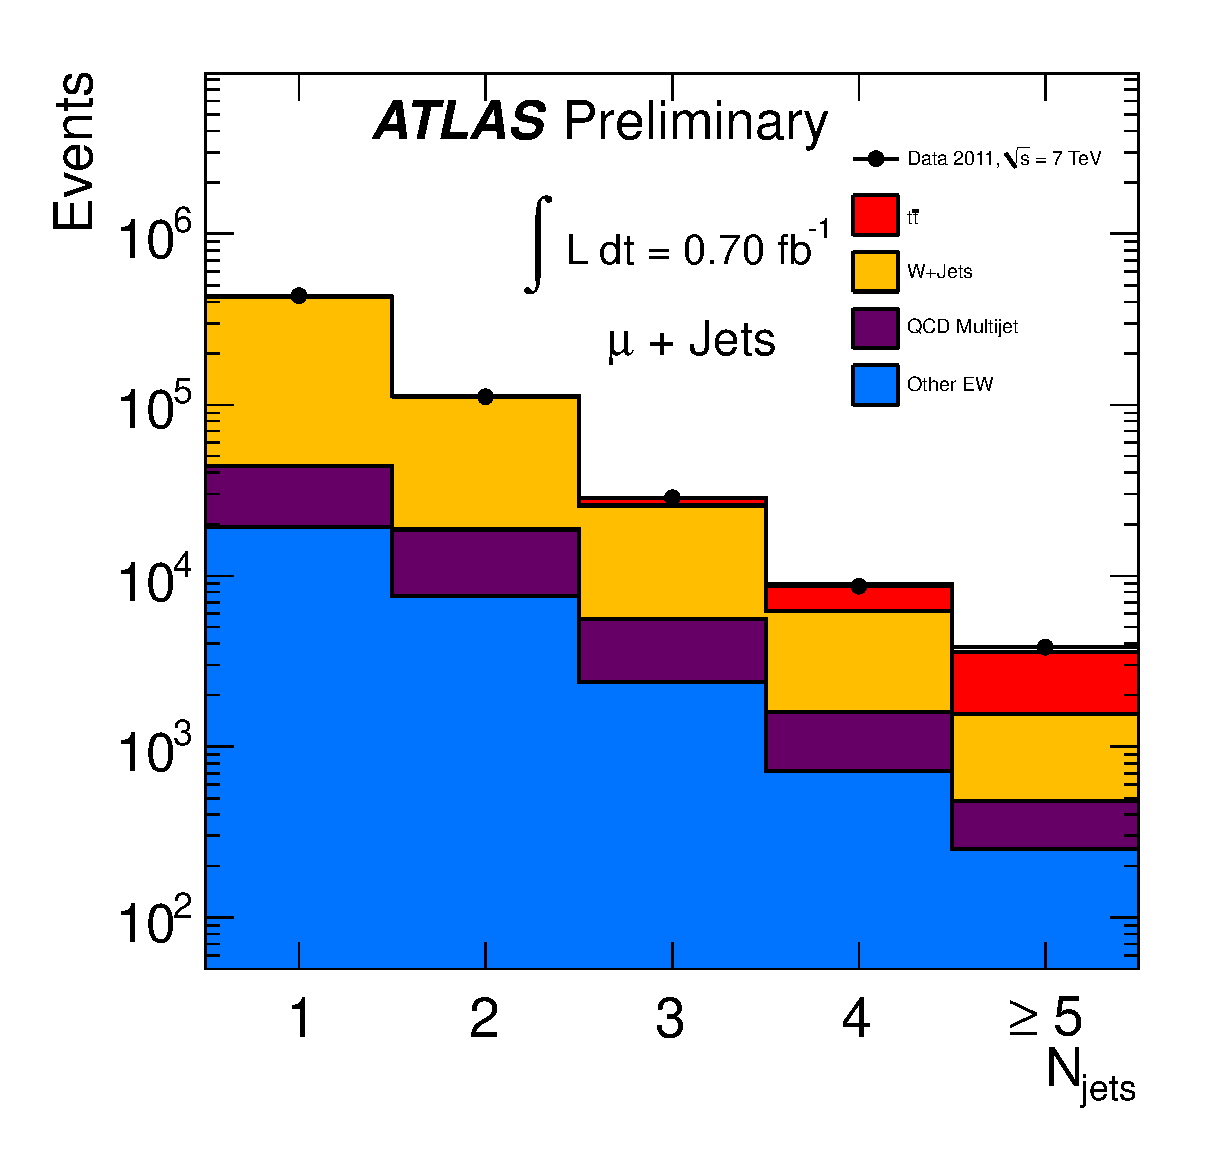
\includegraphics[width=.45\linewidth]{figures/xsection/MuJetsYieldPlot} %  figures/xsection/MuJetsYieldPlots}
    }
  \end{center}
  \caption{The yields of signal and backgrounds in bins of jet number.}
  \label{img:JetNumberYieldPlots}
\end{figure}


% https://atlas.web.cern.ch/Atlas/GROUPS/PHYSICS/CONFNOTES/ATLAS-CONF-2011-121/fig_01a.eps
% https://atlas.web.cern.ch/Atlas/GROUPS/PHYSICS/CONFNOTES/ATLAS-CONF-2011-121/fig_01b.eps


The measurement of the $\ttbar$ cross-section is obtained by fitting multiple multivariate distributions to measured data simultaneously.
These distributions are built out of four kinematic variables: the pseudorapidity of the selected lepton, the $p_{T}$ of the jet with the highest $p_{T}$, the event aplanrity and a variable denoted as $H_{T,3p}$.
The aplanarity, $A$, is defined as 1.5 times the smallest eivenvalue of the matrix

\begin{equation}
  M_{i,j} = \frac{ \sum_{k=1}^{N'_{objects}} p_{ik}p_{jk} }{ \sum_{k=1}^{N'_{objects}} p_{k}^2 }
  \label{eq:Aplanarity}
\end{equation}

and $H_{T, 3p}$, which is the total transverse momentum of all jets except for the first two normalized to the longitudinal momenta of all objects, is given by:

\begin{equation}
  H_{T, 3p} = \frac{ \sum_{i=3}^{N_{jets}} |p_{T, i}| }{ \sum_{j=1}^{N_{objects}} |p_{Z,j}|  }
\end{equation}


\begin{figure}
  \begin{center}
    \subfigure[leading jet $p_{T}$] {
      % DiscrimPtjet4Jets: https://atlas.web.cern.ch/Atlas/GROUPS/PHYSICS/CONFNOTES/ATLAS-CONF-2011-121/fig_04c.eps
      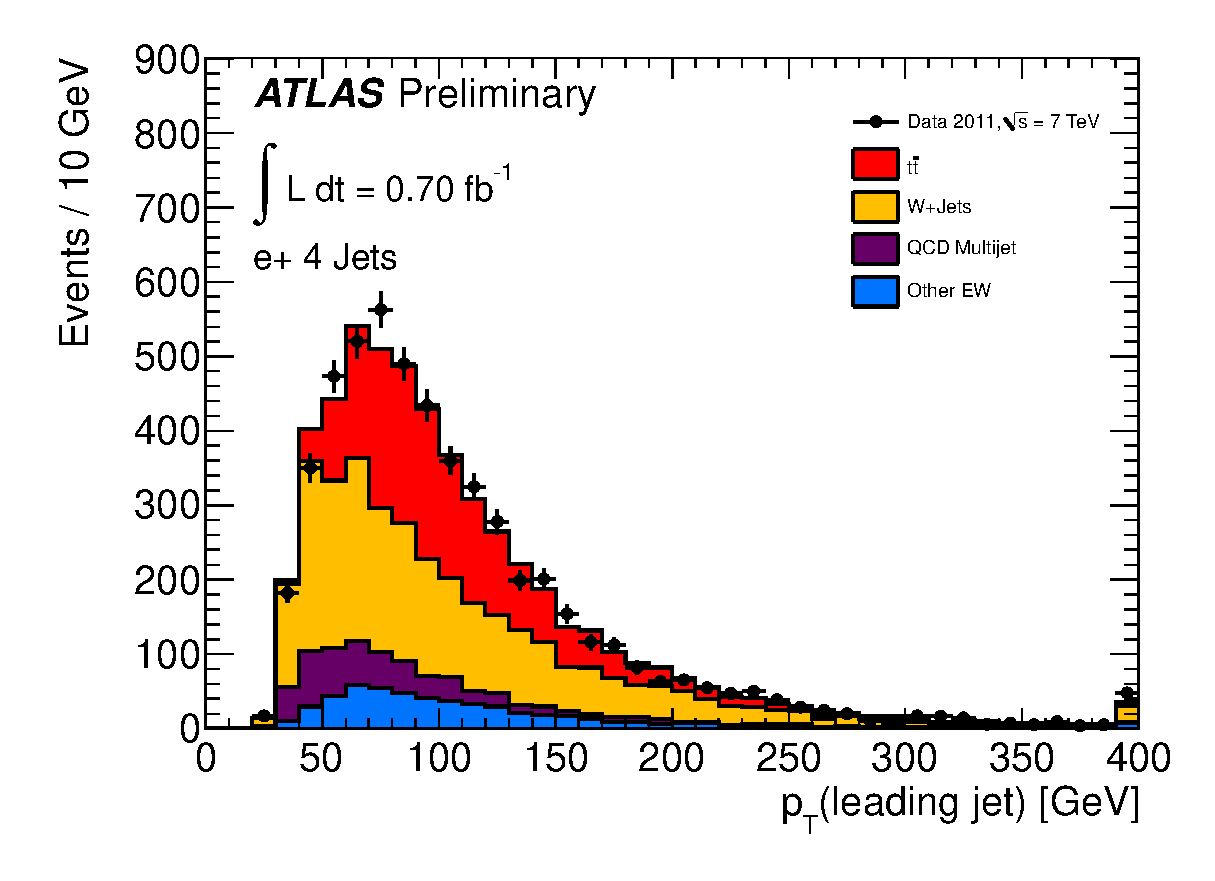
\includegraphics[width=.45\linewidth]{figures/xsection/DiscrimPtjet4Jets}
    }
    \subfigure[lepton ${\eta}$] {
      % DiscrimEtaMu4Jets
      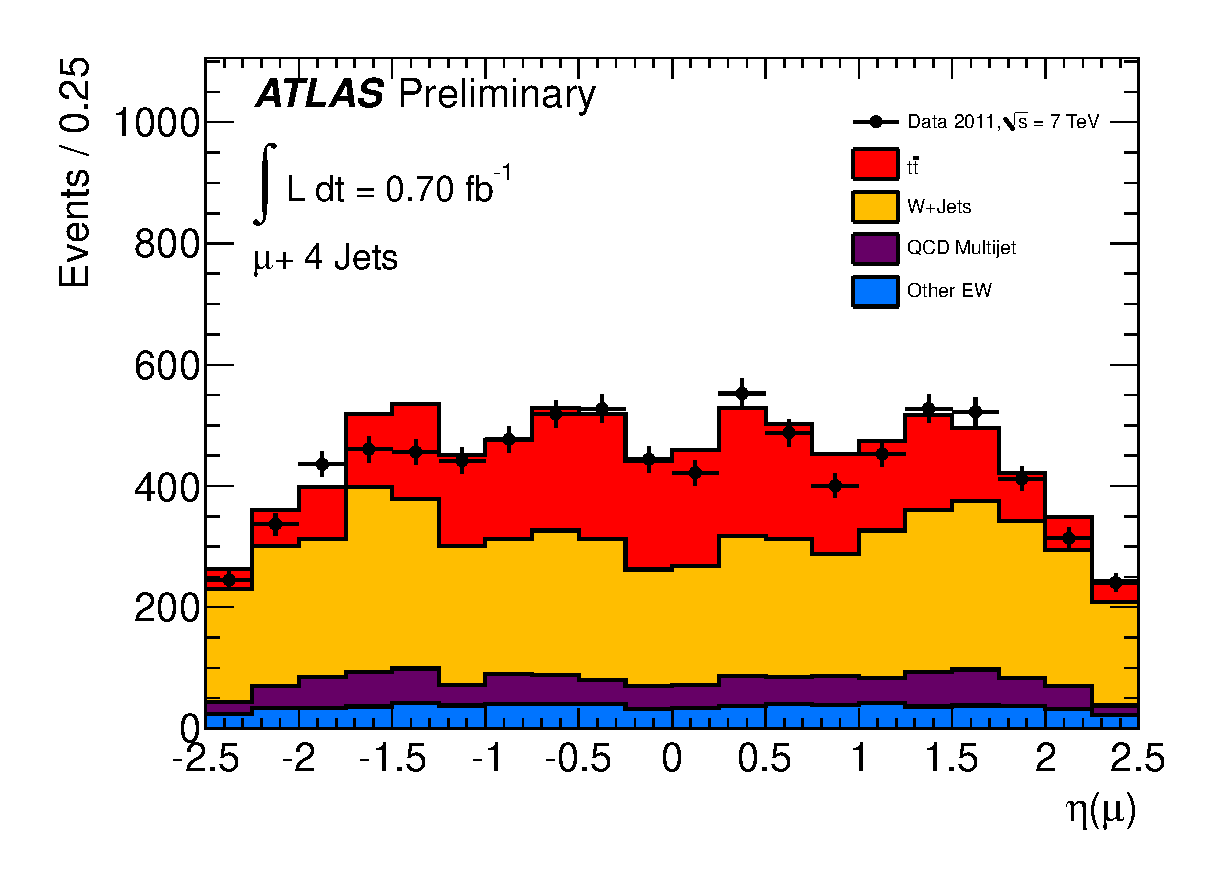
\includegraphics[width=.45\linewidth]{figures/xsection/DiscrimEtaMu4Jets}
    } 
    \subfigure[Aplanarity] {
      % 
      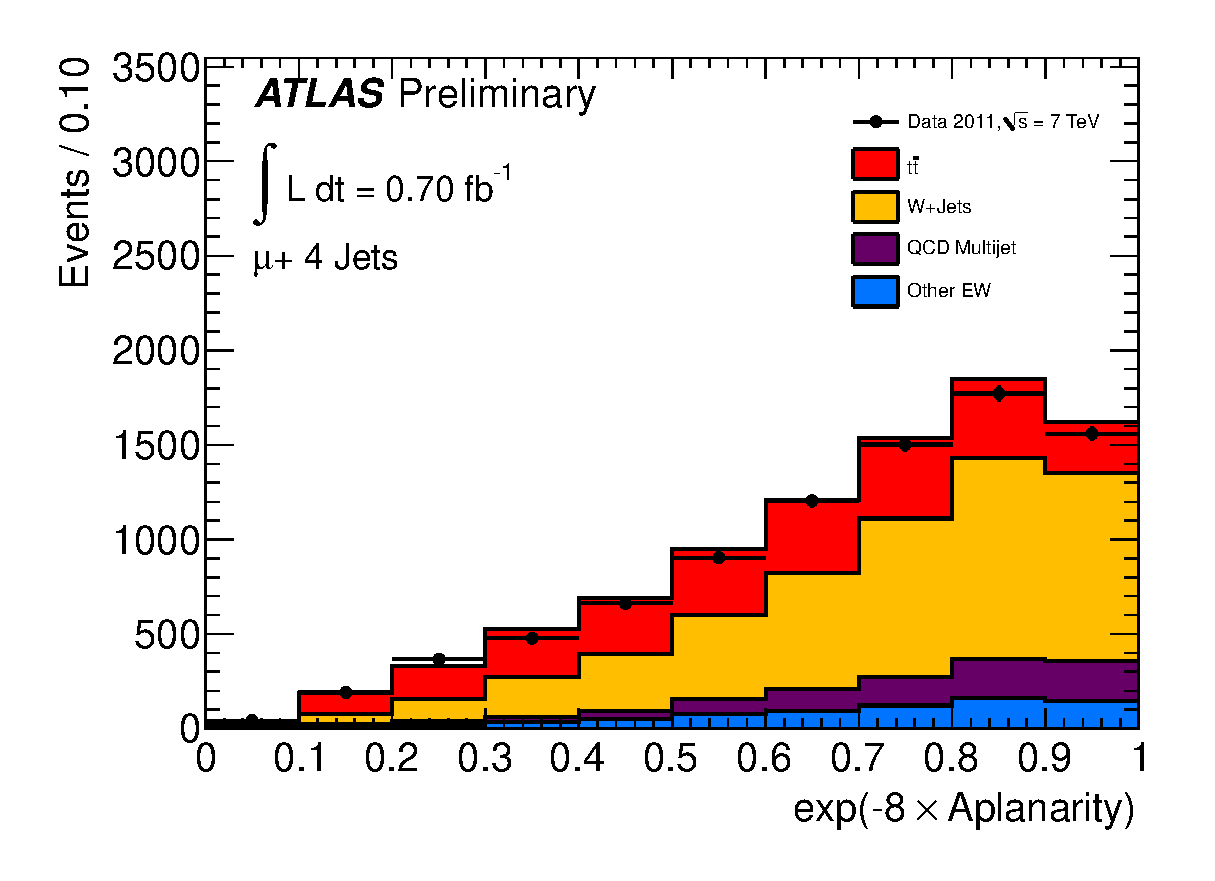
\includegraphics[width=.45\linewidth]{figures/xsection/DiscrimAplanarity4Jets}
    }
    \subfigure[$H_{T,3p}$] {
      % 
      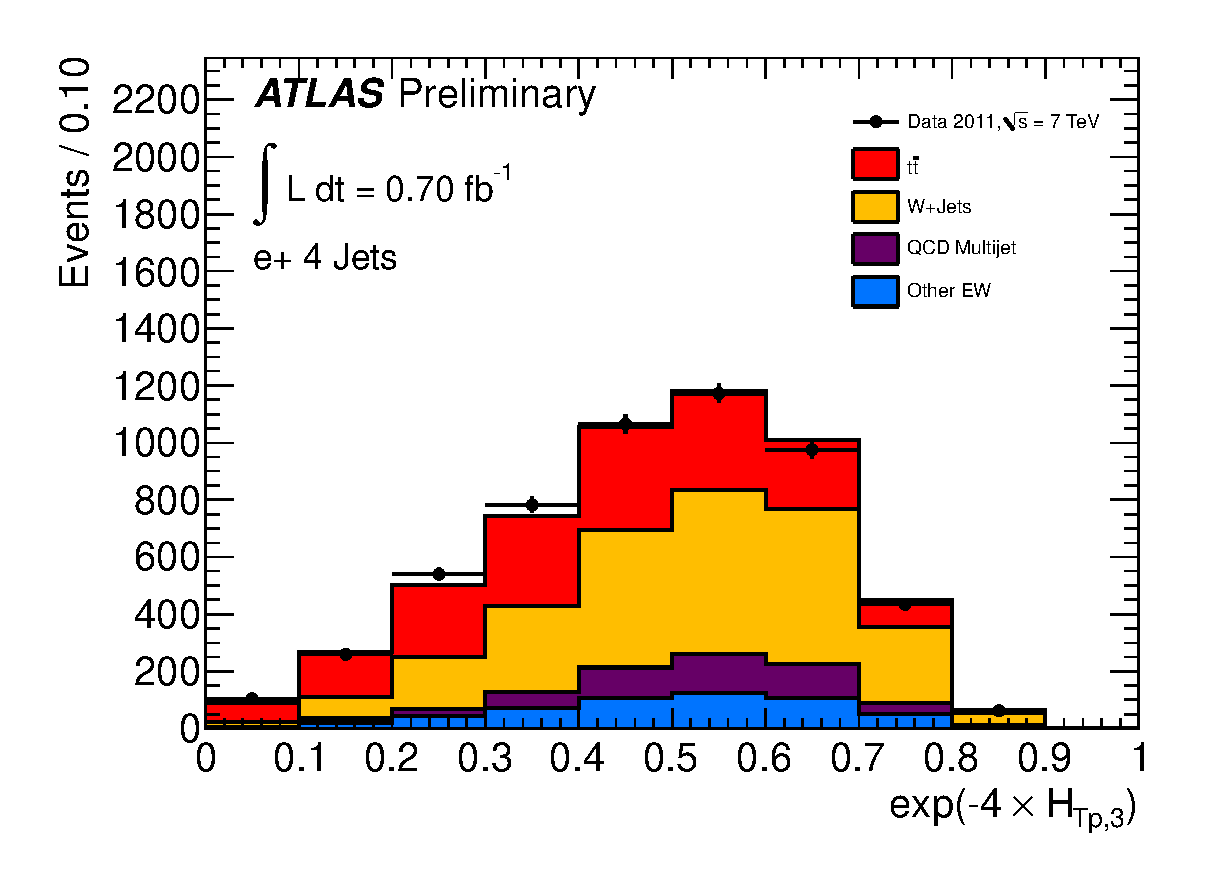
\includegraphics[width=.45\linewidth]{figures/xsection/DiscrimHT34Jets}
    } 
  \end{center}
  \caption{The discriminating variables used in the multivariate likelihood.}
  \label{img:DiscriminatingVariables}
\end{figure}


\begin{figure}
  \begin{center}

    \subfigure[] {
      \includegraphics[width=.95\linewidth]{figures/xsection/LJetsDiscriminantLikelihood}
    }
    \subfigure[] {
      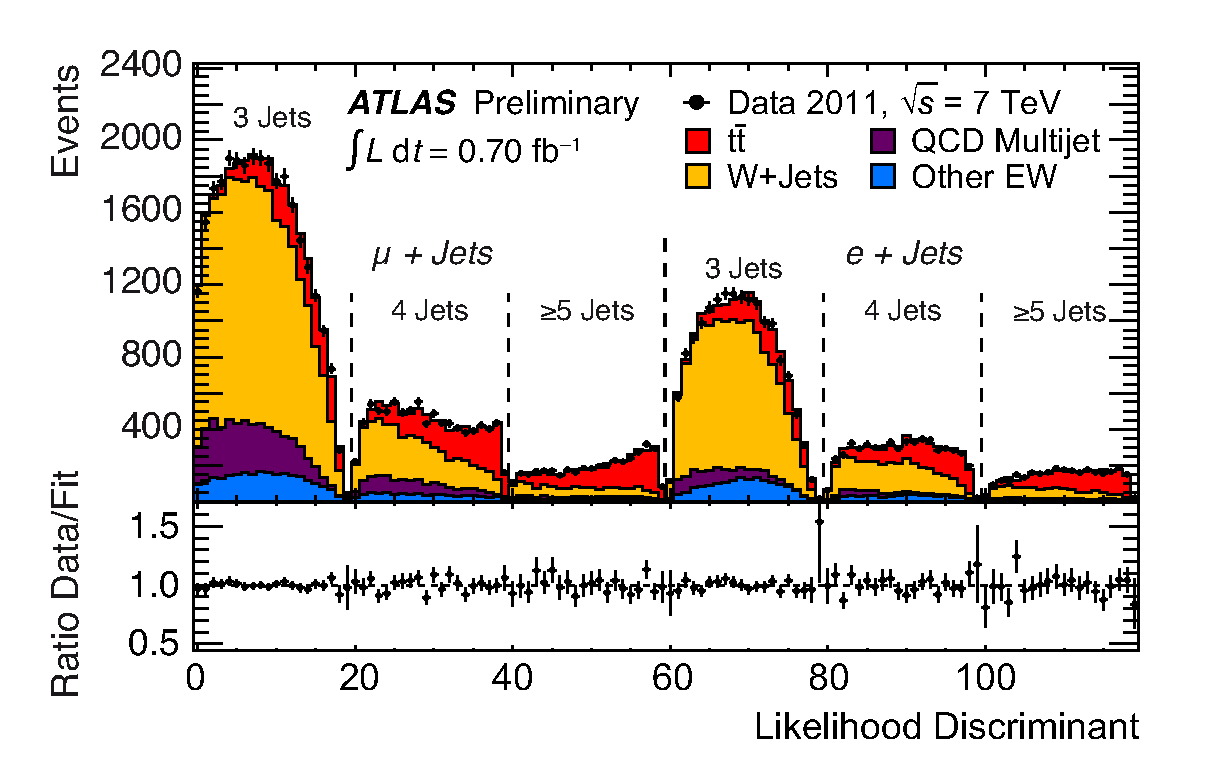
\includegraphics[width=.95\linewidth]{figures/xsection/LJetsFittedLikelihoodDiscriminant}
    }
  \end{center}
  \caption{The multivariate discriminant for $\ttbar$ signal and the dominant $W+Jets$ background.  Distributions are normalized to emphacize the difference in shape between signal and background.}
  \label{img:LJetsLikelihoodDiscriminant}
\end{figure}


\subsection{Systematic Uncertainties}

The careful and consistent of the effect of systematic uncertainties and their proper paramaterization in a likelihood are crucial to making precise measurements.



\subsubsection{Likelihood}

The expected value of the discriminating variable is estimated for every background sample, for every channel, and across all bins.
Using this information, a likelihood function for the measured data in the signal and control regions is created:

\begin{equation}
% L(⃗β, ⃗δ) = 􏰁 P(μk , nk ) × 􏰁 G(β j , ∆ j ) × 􏰁 G(δi , 1)
  L(\vec{\beta}, \vec{\delta}) = \prod Pois(n_{k},\mu_{k}(\vec{\beta},\vec{\delta})) \prod Gauss(\delta_j, \beta_j) \prod( 1, \delta_i),
\end{equation}

where $n_k$ are the values measured in data of each bin of the observable, $\mu_k$ is the expected value of each bin based on a combination of Monte Carlo and data-driven techniques, including the effects of systematic uncertainties.
The systematic uncertainties are paramaterized by two sets of parameters: $\vec{\beta}$, which represent the overall normalizations of backgrounds, and $\vec{\delta}$, which describe various experimental or theoretical uncertainties.

\subsubsection{Results}

This likelihood function, which simultaneously describes all bins across channels for the discriminating variables, is fit to the observed data.
The fitted value of the $\ttbar$ cross section and its uncertainties due to statistical, systematic, and luminosity effects, is found to be $\sigma_{\ttbar} = 179.0 ^{+7.0}_{-6.9}(stat+sys) \pm 6.6 (lumi)$ pb.

Additional uncertainties that are not paramaterized in the Likelihood were added in quadrature to the fitted uncertainties.
These additional uncertainties consist of Generator Hadronization, QCD shape, W shape, and Monte Carlo statistics.

Including these effects, the total uncertainty on the measurement is given by:

$\sigma_{\ttbar} = 179.0 \pm 9.8 (stat + syst) \pm 6.6 (lumi) pb = 179.0 \pm 11.8$ pb.

%%  σtt ̄ =
%% 179.0+7.0 (stat + syst) ± 6.6 (lumi) pb .

%% The combined fit of the six analysis channels to the likelihood discriminant distribution in data in-
%% cluding all systematic uncertainties treated within the fit yields a tt ̄ production cross section of σtt ̄ =
%% 179.0+7.0 (stat + syst) ± 6.6 (lumi) pb . The result of the fit is shown in Fig. 7 and demonstrates an excel- −6.9
%% lent agreement between data and the background and tt ̄ signal model. After including uncertainties that are not part of the fit, σtt ̄ is measured to be
%% σtt ̄ = 179.0±3.9 (stat)±9.0 (syst)±6.6 (lumi) pb = 179.0±9.8 (stat + syst)±6.6 (lumi) pb = 179.0±11.8 pb.


\subsection{Dilepton}


\subsection{Combination}



